\documentclass{article}
\usepackage{amsmath}
\usepackage{graphicx}
\usepackage{float}
\usepackage{bm}
\usepackage{undertilde}
\usepackage[a4paper, total={6in, 9in}]{geometry}
\renewcommand{\familydefault}{\sfdefault}

\title{Evolution of correlation between traits in a sexually recombining population within a single selective environment}
\date{June 2020}
\author{Simon Pirkl, Andreas Rohrbach}

\begin{document}

\maketitle

\begin{center}
	
\includegraphics[height=10mm]{./img/ci/HSWT_Logo_gruen.png}

	\vspace{5mm}
	Department of Bioengineering Sciences, Bioprocess Informatics
\end{center}

% \newpage

\tableofcontents
\newpage

\section{Abstract}

Watson et al. investigated the evolution of phenotypic correlations and "developmental memory". In one of their experiments, an evolutionary model was simulated, containing a single representative individual undergoing individual mutations. This simplification is legit under the assumption of SSWM (strong selection, weak mutation). 
To verify their results in a more realistic model of evolution involving sexual recombination, the experiment was replicated with a more sophisticated fitness evaluation and simple sexual recombination.

It was --Results--

--Discussion--

\section{Introduction}

The phenotypic variants we observe are not purely a product of their genes, but of multiple factors, with developmental processes being one of them \cite{laland2015}. In the work of Watson et al, the evolution of a network of recurrent nonlinear ontogenetic interactions was investigated \cite{watson2014}. Such a network could represent a gene regulation network. In their work, multiple experiments were conducted to better understand the evolution of such networks. In the first experiment, the basic effect of selection on interaction coefficients as a function of a single selective environment was assessed. This experiment was conducted under the assumptions of SSWM (strong selection, weak mutation), under which it is sufficient to model the evolution of just one representative individual undergoing individual mutations. 

One of Watson et al's results is that correlations in their single gene regulation network evolve according to Hebb’s rule \cite{hebb}, a simple associative neural learning mechanism, often summarized as "Cells that fire together wire together" \cite{shatz1992}.
Translated to genes and traits, it would state: if evolution selects a correlation of multiple gene states, those gene states will also become developmentally correlated (see also Pavlicev et al. 2011 \cite{pavlicev2011}).
This could be summarized as "traits that are selected together correlate together" \cite{watson2014}.

We aim to verify their findings in a population context with sexual recombination.
Since mutation and sexual recombination generate greater genetic variation, this could lead to correlations evolving not in accordance with Hebb's rule. However, we postulate that Hebb’s rule is driven not by mutation and recombination, but by selection.
If we reproduce Watson et al’s experiment 1 (single selective environment) for a network population with mutation and recombination, and our adaptive theory is correct, we predict that Hebb’s rule will apply to the evolved networks.

\section{Methods}

The population was modeled ...

\subsection{Gene regulation network}

As in the work of Watson et al, we model our gene regulation network (grn) as a two dimensional matrix $\bm{B}$, containing $nTrait * nTrait$ elements, with $nTrait$ being the number of genes and the number of corresponding traits as well.
Each element of the matrix contains the correlation coefficient between two genes/traits, and is in the range $[-1; +1]$, where 0 corresponds to no correlation at all, a negative coefficient indicating anticorrelation (or negative correlation), and a positive coefficient indicating positive correlation.

-hebb

\subsection{Genotype and phenotype}

The genotype and phenotype are represented by column vectors with $nTrait$ elements. Each element contains a value in the range $[-1; 1]$ which represents the characteristic of the traits.

- magnitude instead of characteristic?
- $\bm{P} and \bm{G}$

Each generation, all genotypes and gene regulation networks are mutated by adding a value in a predefined range to one element of each individual. 
- to one element of each individual -> for genotype and grn
The genotype is mutating faster within the range $[-0.1; 0.1]$ than the gene regulation network, which range is 1/15th of genotype mutation range ($[-0.0067; 0.0067]$).

- which range is 1/15 -> mutational increment?

-lookup: is it really a range or a set?

\subsection{Ontogenetic development}

In every generation the phenotypes have to be developed through time, influenced by the gene regulation network. The starting point is defined by the genotype.

\begin{equation}
	\bm{P}(0) = \bm{G}
\end{equation}

-eq as inline?

After defining the initial phenotype, the development of individuals is represented by simulating through developmental time steps (set at $NDevSteps$ = 10). In each timestep the phenotype experiences the influence of the gene regulation network, calculated by the formula:

- everywhere: individuals -> population frequencies

\begin{equation}
	\bm{P}(t+1) = \bm{P}(t) + \tau_1\sigma(\bm{B}*\bm{P}(t))-\tau_2\bm{P}(t)
\end{equation}

- cite Watson 14 

- sigmoid: tanh

\subsection{Selection and recombination}
- fitness: difference to watson

- selection and recombination



\section{Results}

- for these parameters, this output

- simulation with differing population sizes (common target)

\begin{figure}[H]
	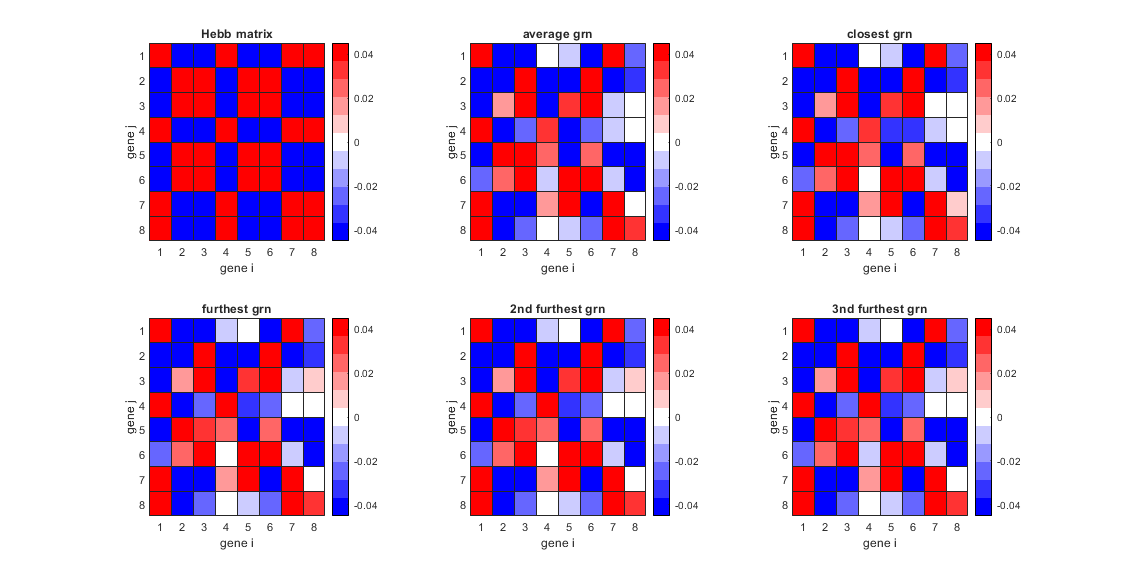
\includegraphics[width=\linewidth]{./img/dummy.jpg}
	\caption{This is just a dummy graphic}
	\label{fig:dummy}
\end{figure}


\section{Discussion}

- interpret results

- so much gentic variation, that genes are more important than grn?

- from where parameters like 1/15 for mutational rate of gene to grn?

- when in later generations more frequencies are quite fit, maybe the selective pressure should increase to reach even better grns ?

- more experiments from watson14 should be verified with this more realistic model of evolution

- Sniegowskiand Murphy 2006 ???

- could we really achive good grns faster? since in 1 generation, watson have 1 mutation, we have nPop mutations.... 


\section{Stuff / Ideas / Todos}

\subsection{Topic}
\subsubsection{Research question}
Watson et al derive their results from an evolutionary model containing a single representative individual undergoing individual mutations, motivating this model from the assumption of SSWM (strong selection, weak mutation). Do their results still hold in a more realistic model of evolution involving sexual recombination?

\subsubsection{Adaptive theory}
Watson et al’s central result is that correlations in their single gene regulation network evolve according to Hebb’s rule: if evolution selects a correlation of multiple gene states, those gene states will also become developmentally correlated. Since mutation and sexual recombination generate greater genetic variation, this could lead to correlations evolving not in accordance with Hebb's rule. However, we postulate that Hebb’s rule is driven not by mutation and recombination, but by selection.

\subsubsection{Research hypothesis}
If we reproduce Watson et al’s experiment 1 (single selective environment) for a network population with mutation and recombination, and our adaptive theory is correct, we predict that Hebb’s rule will apply to the evolved networks.

% \subsection{cheat sheet}
% include a graphic:

% \begin{figure}[h!]
% 	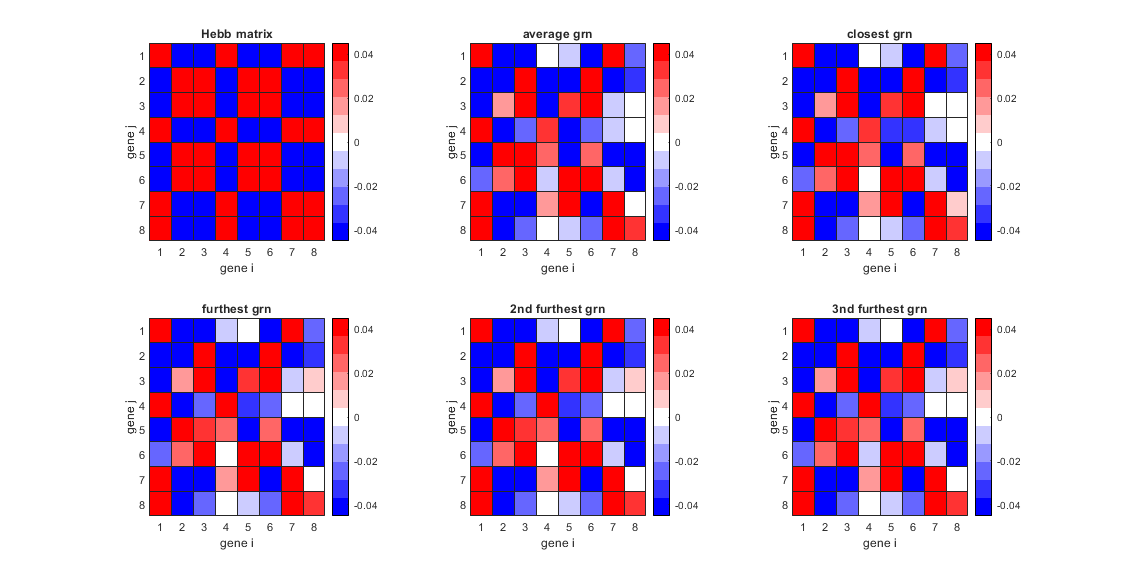
\includegraphics[width=\linewidth]{./img/dummy.jpg}
% 	\caption{This is just a dummy graphic}
% 	\label{fig:dummy}
% \end{figure}


% some inline math: $f(x) = \sqrt{4*\pi}$ , or not:
% \begin{equation}
% 	f(x) = \frac{x^2}{7x}
% \end{equation}

% matrices:
% \begin{equation}
% \left[
% \begin{matrix}
% 1 & 0 & 1\\
% 0 & 1 & 0
% \end{matrix}
% \right]
% \end{equation}

% \newpage


\begin{appendix}
  \listoffigures
  \listoftables
  \bibliography{Bericht} 
  \bibliographystyle{ieeetr}
\end{appendix}

\end{document}
